\chapter{Practical Operation} 
\label{chapter:practical-op}
\begin{figure}[!h]
 \centering
 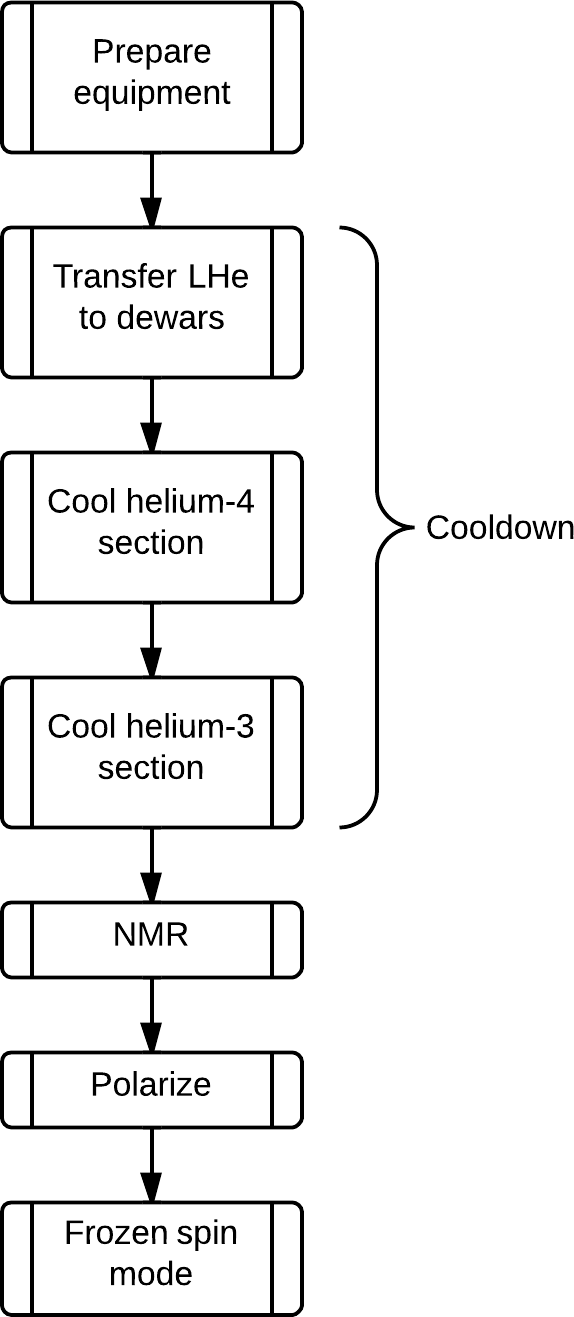
\includegraphics[scale=.24]{./img/cooldown-overview-flowchart.png}
 % cooldown-overview-flowchart.png: 102x490 pixel, 100dpi, 2.59x12.45 cm, bb=0 0 73 353
 \caption{Practical steps to polarize target material with HiFrost.}
 \label{fig:cooldown-overview-flowchart}
\end{figure}

This chapter assumes the reader is familiar with everything safety related.  Read Chapter \ref{safety} before attempting anything here.



\section{Cooldown Prep and LHe Filling}
\subsection{Prep}
\label{practical-op:prep}
Go down the checklist found in Appendix \ref{appendix:checklist-for-cooldown}, reporting any issues to the senior cooldown scientist.

\textbf{This step is not optional}: the rest of this operational procedure assumes all prep work is successfully completed and equipment bugs are worked out.  See walkthroughs for specifics tasks in Chapter \ref{procedures}.

\section{LHe Transfer}

Figure \ref{fig:cryo-schematic-all} is a schematic of the LHe transfer system.  More detailed figures of the dewars are found later in the chapter, and complete technical drawings of the TLs are found in Appendix \ref{appendix:tl-drawings}.

\begin{figure}[htbp!]
 \centering
 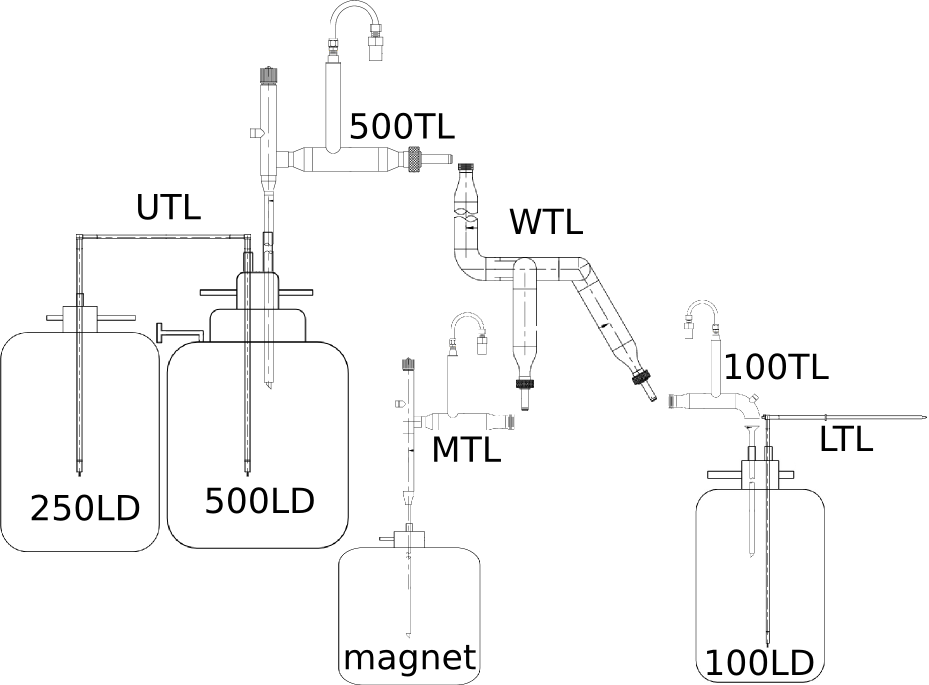
\includegraphics[width=\textwidth]{./img/cryo-schematic-all.png}
 % cryo-schematic-all.png: 0x0 pixel, 0dpi, 0.00x0.00 cm, bb=
 \caption{Schematic overview of the LHe transfer and storage system.}
 \label{fig:cryo-schematic-all}
\end{figure}

\subsection{Dewar Filling}
The 500LD and 100LD are initally filled before cooling the fridge.  The magnet is filled either before or after dilution.

The 250LD has an LHe outlet port, a pressurization/exhaust port and the pressure relief port, shown in Figure \ref{fig:250LD-cartoon}.  Each port has an accompanying valve.

The 500LD has an inlet port (for LHe filling and the level probe), an outlet port, a pressurization port, a vacuum pump out port and a pressure relief port, as shown in Figure \ref{fig:500LD-cartoon}.  Only the pressurization, vacuum pump out and pressure relief ports have accompanying valves.


\begin{figure}[!htbp]
\centering
 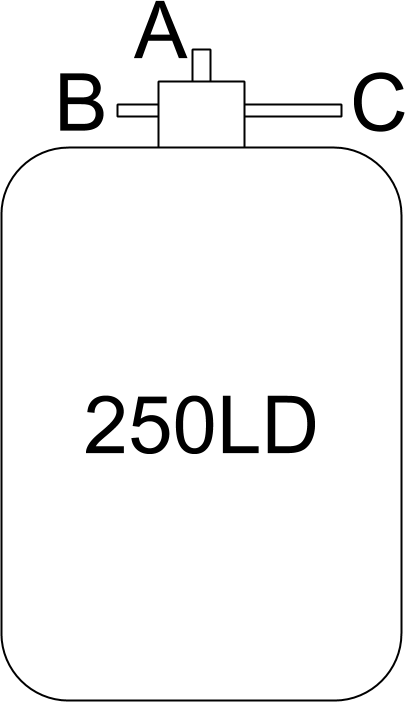
\includegraphics[width=.25\textwidth]{./img/250LD-cartoon.png}
 % 500LD-cartoon.pdf: 0x0 pixel, 0dpi, nanxnan cm, bb=
 \caption{An example of 250LD ports: A) LHe outlet port, B) pressure relief valve, C) pressurization/exhaust port.}
 \label{fig:250LD-cartoon}
\end{figure}


\begin{figure}[!htbp]
 \centering
 \begin{minipage}{.35\textwidth}
 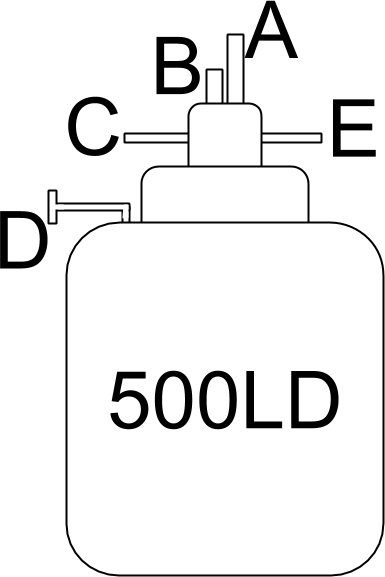
\includegraphics[width=\textwidth]{./img/500LD-cartoon.png}
 % 500LD-cartoon.pdf: 0x0 pixel, 0dpi, nanxnan cm, bb=
 \caption{The 500LD ports.}
 \label{fig:500LD-cartoon}
 \end{minipage}
 \quad
  \begin{minipage}{.50\textwidth}
 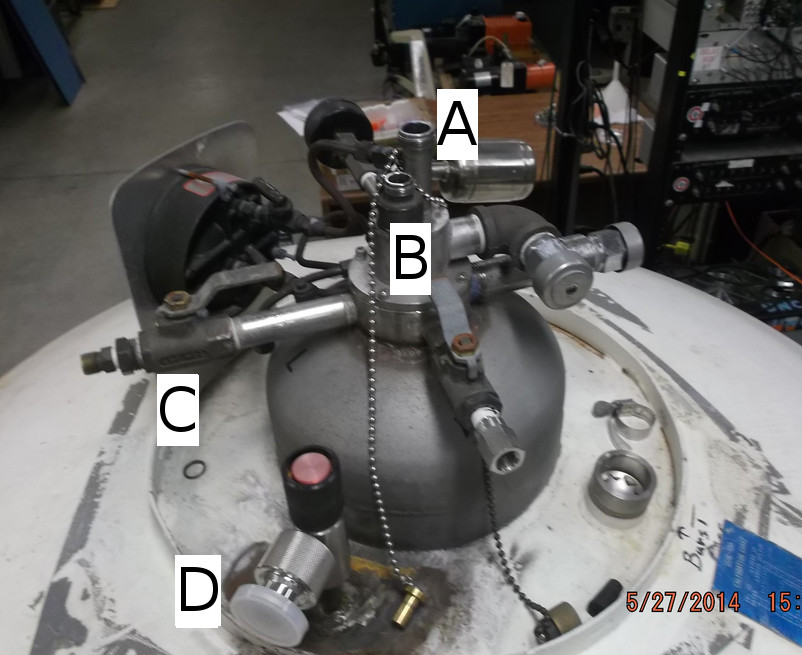
\includegraphics[width=\textwidth]{./img/500LD-photo.jpg}
 % 500LD-cartoon.pdf: 0x0 pixel, 0dpi, nanxnan cm, bb=
 \caption{Photo of 500LD: A) LHe inlet port, B) LHe outlet port, C) pressurization port, D) vacuum pump out port, E) pressure relief valve.}
 \label{fig:500LD-photo}
 \end{minipage}
 \end{figure}

\pagebreak



\subsection{500LD Fill}
\label{practical-op:500LDfill}
\begin{enumerate}
 \item Weigh a full 250LD according to the procedure in Section \ref{weigh-250LD} before breaking the seal on it.
 \item Check 250LD level using the procedure in Section \ref{procedure:check-lhe-level}.
 \item Place correct Goddard fittings on the 250LD and/or the UTL.
 \item Blow out UTL with helium gas by fitting the universal hose over it and putting about 2 PSI on the helium cylinder. \label{procedure:500LDfill-blowoutUTL}
 \item $[$\textbf{initial 500LD fill only}$]$ Purge the 500LD with helium gas by hooking up the pressurization line, closing the main flow valve, opening the pressure release valve and putting 5 pounds of pressure on the 500LD for about 10 minutes (Figure \ref{fig:500LDfill-02-blow-out-500LD}).  Remove the pressurization line. \label{procedure:500LDfill-purge500LD}%for some godforsaken reason square brackets have to be in math mode to not ruin enumerated lists
 \item Open main flow valve on 500LD to vent pressure (if any), then open pressurization valve making sure the pressurization port is not pointed at anyone.
 \item Release the 250LD pressure from the main flow valve and close the pressure relief valve.  Slowly lower the correct end of the UTL down into the 250LD about 30 cm or until helium gas is blowing out the 500LD end, as shown in the left side of Figure \ref{fig:500LDfill-03-04-insert-UTL-in-250LD-and-500LD}.  Then, lower the 500LD end in as far as it can go, while continuing to slowly lower the 250LD side at a rate of about 2 cm/s.  A cold plume should be coming out of the 500LD.  Check that no gas is escaping through the Goddard fittings on either dewar (if it is, replace fitting o-rings). \label{procedure:insert-UTL-in-250LD}
 \item Hook up the pressurization line to the 250LD pressurization port using the procedure in Section \ref{procedure:attach-pressurization-line} and open the pressurization valve as shown in the right side of Figure \ref{fig:500LDfill-03-04-insert-UTL-in-250LD-and-500LD}.  There should now be 2 PSI on the 250LD. \label{procedure:insert-UTL-in-500LD}
 \item Periodically measure the 250LD level using the procedure in Section \ref{procedure:check-lhe-level}.  When it is empty, stop flow from the pressurization cylinder regulator and disconnect the pressurization line.
 \item Simultaneously raise both sides of the UTL out of the dewars and hang it on the wall to warm up.
 \item Bung the 500LD inlet port, close the 500LD pressurization valve, and leave open the pressure relief valve.
 \item On the 250LD, open the pressure release valve and close the main flow and pressurization valves.
 \item Recover the Goddard fittings from the 250LD and bring it back to the weigh area.  Record the final weight on the log sheet.
\end{enumerate}

\begin{figure}[htbp!]
 \centering
 \begin{minipage}{.47\textwidth}
 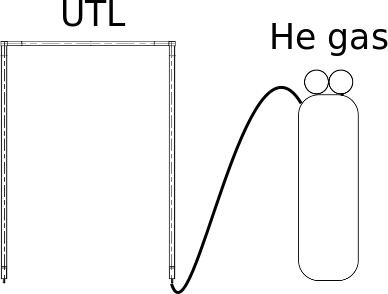
\includegraphics[width=\textwidth]{./img/500LDfill-01-blow-out-UTL.png}
 \caption{Blowing out the UTL with He gas (Step \ref{procedure:500LDfill-blowoutUTL}).}
 \label{fig:500LDfill-01-blow-out-UTL}
 \end{minipage}
 \quad
 \begin{minipage}{.47\textwidth}
 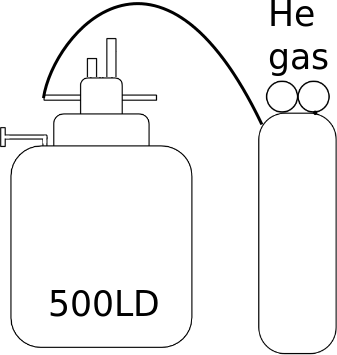
\includegraphics[width=\textwidth]{./img/500LDfill-02-blow-out-500LD.png}
 \caption{\textbf{Initial 500LD fill}, purging the 500LD with He gas (Step \ref{procedure:500LDfill-purge500LD}).}
 \label{fig:500LDfill-02-blow-out-500LD}
 \end{minipage}
\end{figure}

\begin{figure}[htbp!]
 \begin{minipage}{.38\textwidth}
 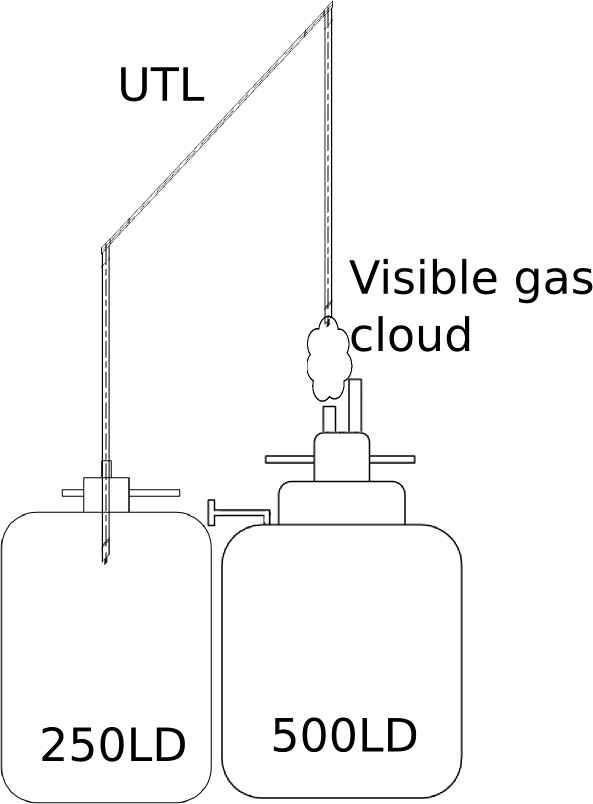
\includegraphics[width=\textwidth]{./img/500LDfill-03-insert-UTL-in-250LD.png}
 \end{minipage}
  \quad
 \begin{minipage}{.58\textwidth}
 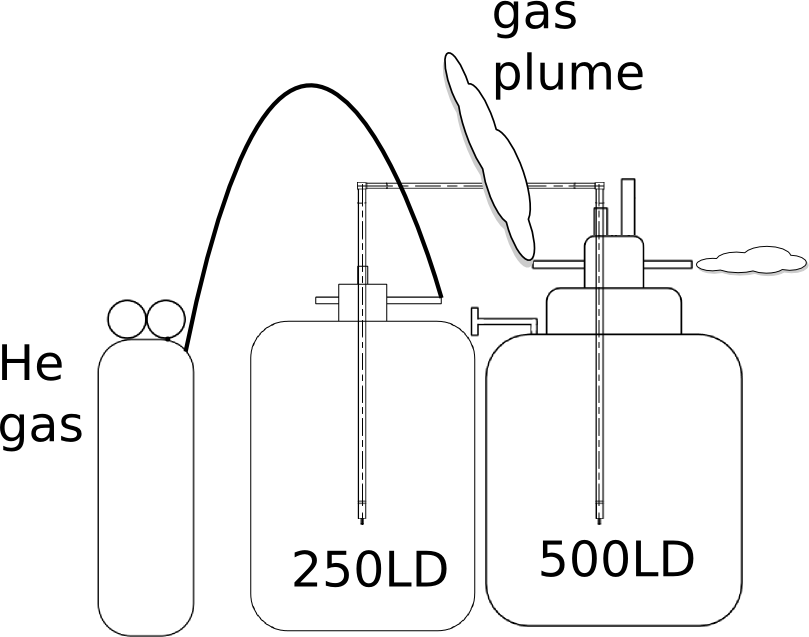
\includegraphics[width=\textwidth]{./img/500LDfill-04-insert-UTL-in-500LD.png}
 \end{minipage}
 \caption{Inserting the UTL first in the 250LD, then the 500LD, as described in Steps \ref{procedure:insert-UTL-in-250LD} and \ref{procedure:insert-UTL-in-500LD}.  The pressurization line is attached to the 250LD to facilitate liquid transfer.}
 \label{fig:500LDfill-03-04-insert-UTL-in-250LD-and-500LD}
 \end{figure}
 
\pagebreak

\subsection{Initial 100LD Fill}

The 100LD has an entrance port, a main flow port, an exhaust port and a pressure relief port.  The exhaust and pressure relief ports have accompanying valves.
 
 \begin{figure}[!htbp]
 \centering
 \begin{minipage}{.55\textwidth}
 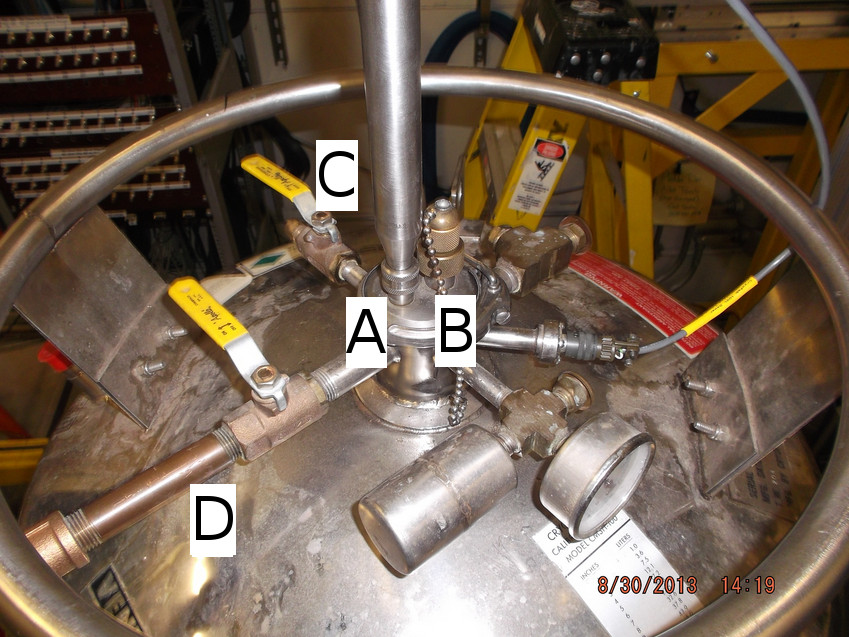
\includegraphics[width=\textwidth]{./img/100LD-photo.jpg}
 % 500LD-cartoon.pdf: 0x0 pixel, 0dpi, nanxnan cm, bb=
 \caption{Photo of 100LD: A) LHe inlet port, B) LHe outlet port, C) pressure relief valve, D) pressurization/exhaust port.}
 \label{fig:100LD-photo}
 \end{minipage}
 \quad
  \begin{minipage}{.40\textwidth}
 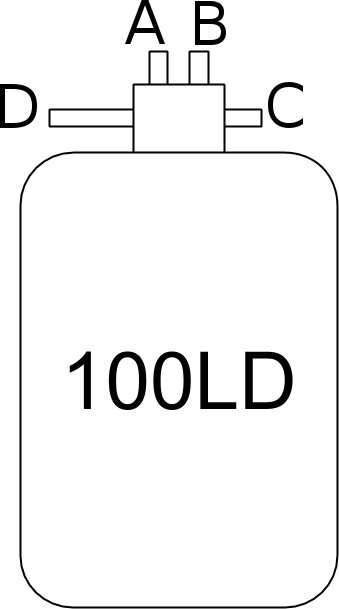
\includegraphics[width=\textwidth]{./img/100LD-cartoon.jpg}
 % 500LD-cartoon.pdf: 0x0 pixel, 0dpi, nanxnan cm, bb=
 \caption{100LD cartoon.}
 \label{fig:100LD-cartoon}
 \end{minipage}
 \quad
\end{figure}



\begin{figure}[htbp!]
 \centering
 \begin{minipage}{.48\textwidth}
 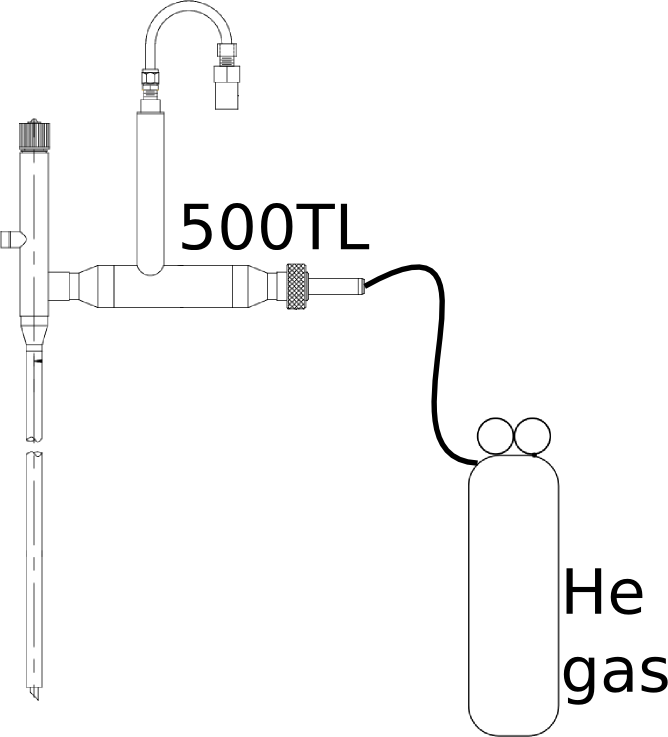
\includegraphics[width=\textwidth]{./img/100LDfill-01-blow-out-500TL.png}
 \label{fig:100LDfill-01-blow-out-500TL}
 \end{minipage}
 \quad
 \begin{minipage}{.48\textwidth}
 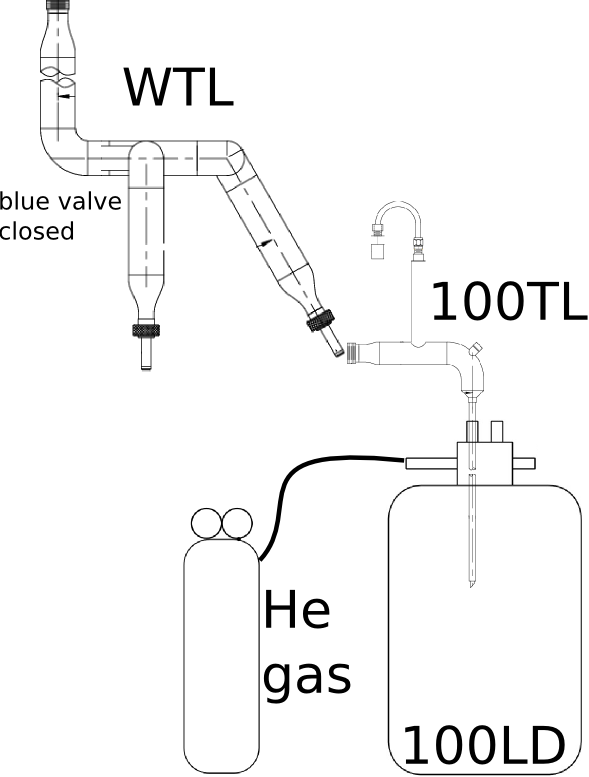
\includegraphics[width=\textwidth]{./img/100LDfill-02-blow-out-WTL.png}
 \label{fig:100LDfill-02-blow-out-WTL}
 \end{minipage}
 \caption{Blowing out the 500TL and WTL.}
\end{figure}


\begin{figure}[htbp!]
 \centering
 \begin{minipage}{\textwidth}
 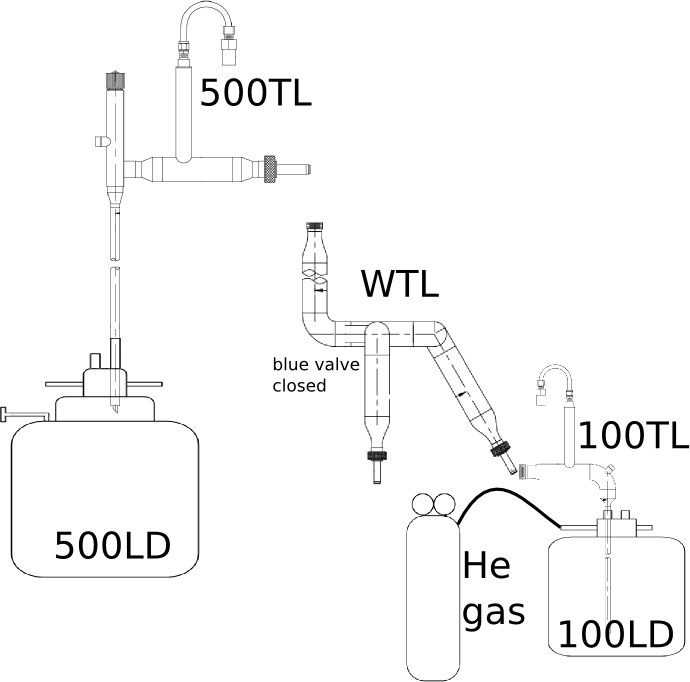
\includegraphics[height=.45\textheight]{./img/100LDfill-03-insert-500TL.png}
 \caption{Lower the 500TL in the 500LD about 30 cm.}
 \label{fig:100LDfill-03-insert-500TL}
 \end{minipage}
 \begin{minipage}{\textwidth}
 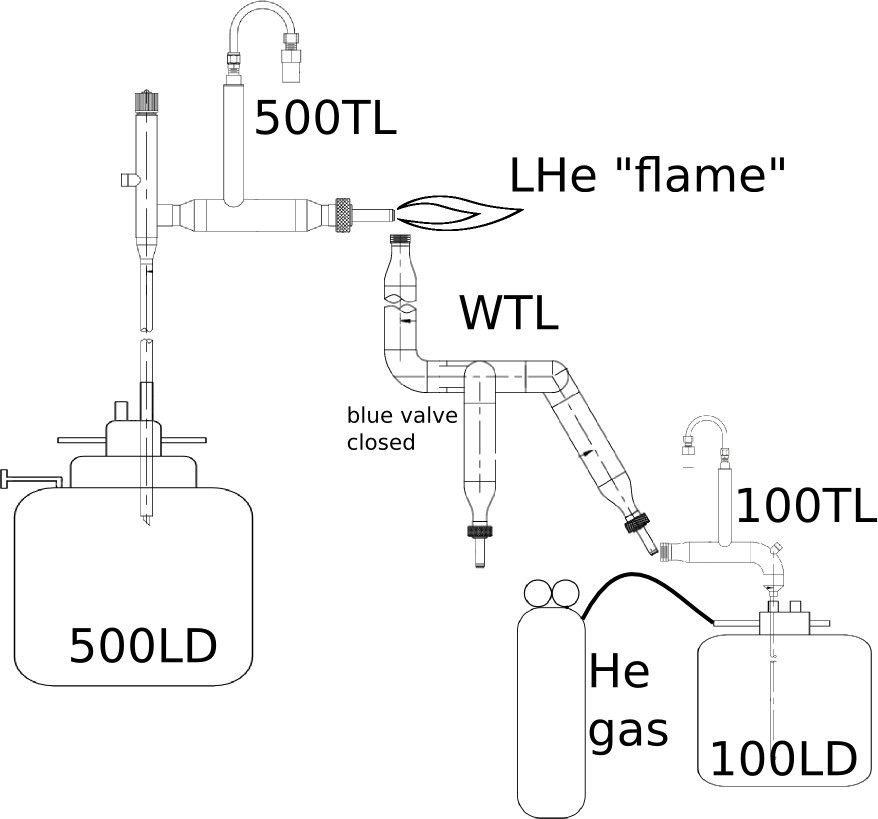
\includegraphics[height=.45\textheight]{./img/100LDfill-04-insert-500TL.png}
 \caption{Lower the 500TL until the bayonet reaches the WTL.}
 \label{fig:100LDfill-04-insert-500TL}
 \end{minipage}
 \end{figure}

 \begin{figure}[htbp!]
 \centering
 \begin{minipage}{\textwidth}
 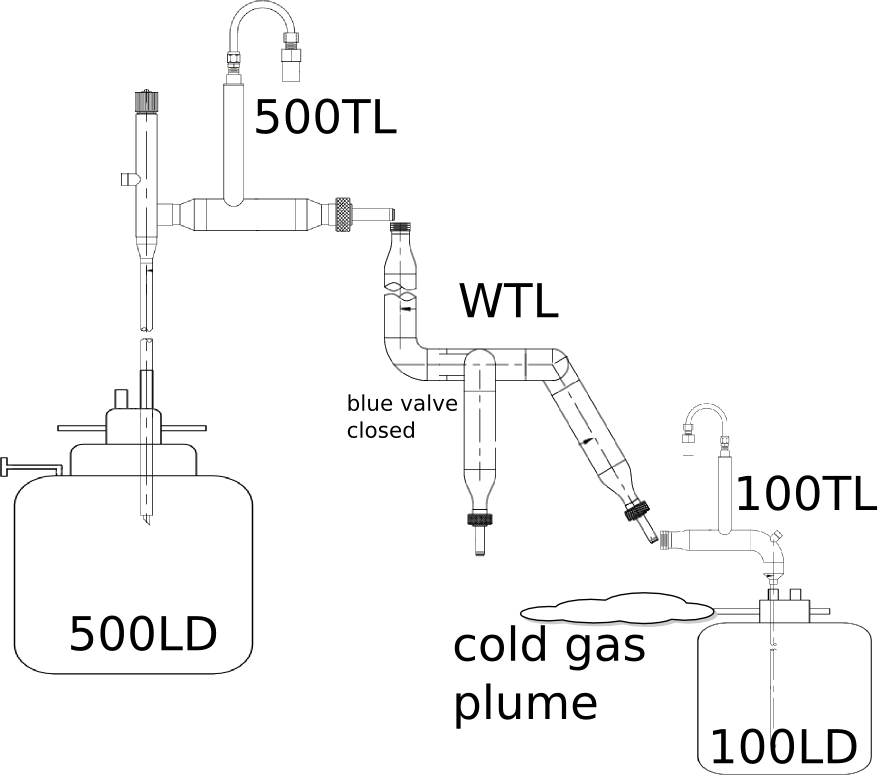
\includegraphics[height=.40\textheight]{./img/100LDfill-05-insert-500TL.png}
 \caption{Insert the 500TL into the WTL and immediately remove pressure from the 100LD to exhaust the cold gas plume.}
 \label{fig:100LDfill-05-insert-500TL}
 \end{minipage}
 \quad
 \begin{minipage}{\textwidth}
 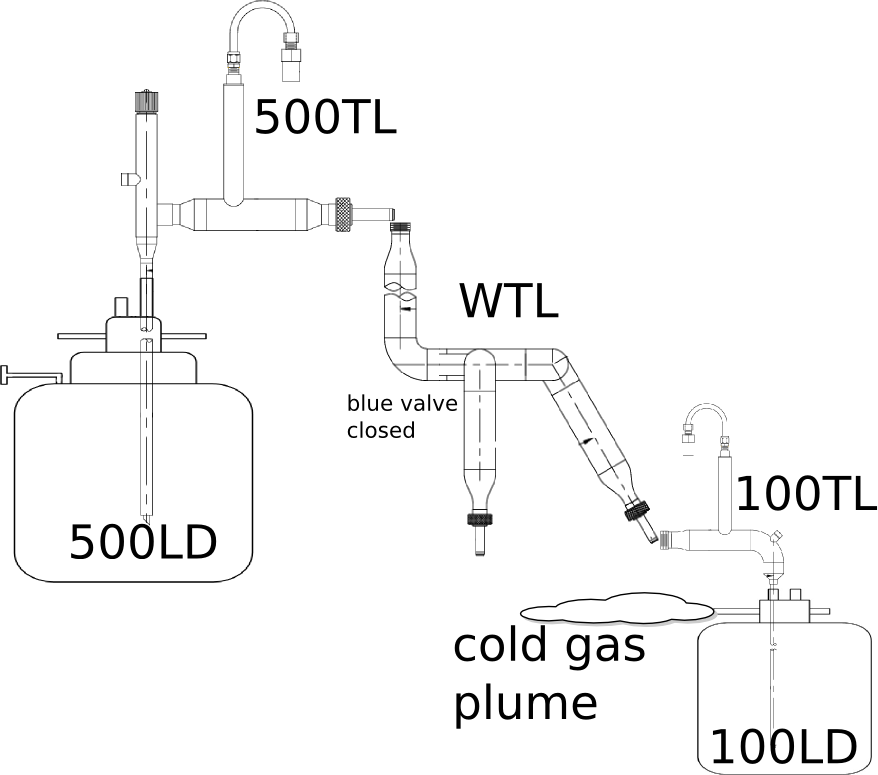
\includegraphics[height=.45\textheight]{./img/100LDfill-06-insert-500TL.png}
 \caption{Finish lowering the 500TL into the 500LD.}
 \label{fig:100LDfill-06-insert-500TL}
 \end{minipage}
\end{figure}

\begin{enumerate}
 \item Purge the 500TL with helium gas (with the shutoff valve open).
 \item Close the magnet LHe inlet valve on the WTL (blue valve).
 \item Open the 100LD exhaust valve, close the pressure release valve and bung the main flow valve.
 \item Uncap WTL by the pump station area.
 \item Hook up the universal He gas line in the GV to the 100LD exhaust port and pressurize to 2 PSI.
 \item Verify the positive pressure on the WTL by the pump station.  Increase the helium cylinder pressure if necessary.  Wait 10 minutes for the 100LD, 100TL and WTL to purge.
 \item Close the 500TL shutoff valve and stop purging it.
 \item Vent the 500LD through the pressurization port so as not to freeze the Goddard fittings.
 \item Unbung the 500LD LHe outlet port.
 \item Close the 500LD pressurization and pressure relief valves.
 \item Slowly lower the 500TL about 30 cm.
 \item Open the 500TL shutoff valve about half a turn.
 \item While watching the gas coming out of the 500TL, slowly lower the 500TL in the 500LD until the bayonet can reach the WTL.
 \item Open the 500TL shutoff valve the rest of the way.  When the plume looks like a blowtorch, attach the 500TL to the WTL and tighten.
 \item \textbf{Immediately remove the pressurization line from the 100LD exhaust port and open the 100LD pressure relief valve.} Verify gas is coming out the exhaust.
 \item Slowly lower the 500TL all the way down into the 500LD and tighten the Goddard fitting.  Use the heat gun if the Goddard fitting freezes before the 500TL is completely in.
 \item Hook up the pressurization line to the 500LD pressurization port using the procedure in Section \ref{procedure:attach-pressurization-line} and open the 500LD pressurization valve.
 \item Turn on the 100LD level probe and monitor the liquid level.
 \item When the 100LD is full there will be a large white plume coming from the exhaust and the level probe will read around 24.9 (arbitrary units). Close the 500LD pressurization valve.
 \item Open the 500LD pressure relief valve.
 \item Close the 500TL shutoff valve.
 \item Close the 100LD exhaust valve.
\end{enumerate}

\pagebreak


\subsection{100LD Fill During Run}

\begin{enumerate}
 
 \item Verify the 500LD has enough LHe to top off the 100LD.
 \item Set the regulator on the helium pressurization cylinder to 2 PSI.
 \item Open the 100LD exhaust and pressure relief valves.
 \item Hook up the pressurization line to the 500LD using the procedure in Section \ref{procedure:attach-pressurization-line}.
 \item Open the shutoff valve on the 500TL
 \item Close the 500LD pressure relief valve.
 \item Open the 500LD pressurization valve.
 \item Verify the 100LD Goddard Fittings are tight.  If not, remove the pressurization from the 500LD and close the 500TL main flow valve immediately.  Consult a high ranking lab official.
 \item When the 100LD is full, close the 500LD pressurization valve.
 \item Open the 500LD pressure relief valve.
 \item Close the 500TL shutoff valve.
 \item Close the 100LD exhaut valve.
 
\end{enumerate}

\pagebreak

\subsection{Cool \hef{} Section}

When the 100LD is full, the fridge has been backfilled with helium gas and the rest of the system is ready for a cooldown, the LTL is inserted into the 100LD and fridge.  The separator pumps on the fridge are started and the pressure difference is enough to pull helium from the 100LD (no dewar pressurization needed).

The LHe travels through the LTL into the separator, which collects liquid while rejecting gas.  The gas is pulled out through two lines, the ``separator'' line which precools the \het{} inlet, and the shield line which provides a heat shink for the radiation shield.

When the separator is full, control valve 1 (CV1) allows helium to flow to the evaporator and control valve 2 (CV2) directs LHe to the holding magnet and IVC can.  CV2 is also used to quickly cool the MC when target material is at risk of thermal damaged.

The evaporator can hold LHe at 4K, but evaporator pumps are run to lower the helium vapor pressure and lower the temperature down to a minimum of about 1K.

\subsection{Insert LTL}
\begin{enumerate}
 \item See Section \ref{practical-op:prep} to make sure the fridge is ready to take LHe.
 \item Check the 100LD level probe and top off if necessary (see directions above).
 \item Blow out LTL with helium gas.
 \item Make sure 100LD can roll out from under the fridge stand area (so the LTL can be inserted), back under the fridge stand area, and then up to the fridge.  The IVC pump cart may have to be shifted around.
 \item Put 4 PSI on the fridge via the following steps: adjust the helium gas regulator to 4 PSI, open the valves between the regulator and the separator manifold, close all other separator manifold valves (so gas does not flow to separator pumps).
 \item Remove the LHe inlet bung and KF clamp from the fridge and verify the positive pressure from the separator.
 \item Stop purging LTL with gas and place a rubber in the fridge side.
 \item Remove bung from 100LD main flow port and slowly insert the LTL until it lines up with the fridge.
 \item Roll the 100LD in place under the fridge stand.
 \item Remove the LTL bung and wait for the gas plume to look like a blue torch flame, then roll the 100LD towards the fridge until the LTL is fully inserted and tighten the KF clamp around the LTL-fridge inlet joint.
 \end{enumerate}
 
 \subsection{Cool Separator}
 \begin{enumerate}
 \item Open CV1 and CV2 about 2 turns each.
 \item Immediately turn off the pressurization from the helium cylinder and turn on the separator pumps.  Open all valves between the separator pumps and the fridge, including bypass valves.  Pump on shield at max flow for 30 minutes and separator for 15 minutes\cite{tapio-cooldown-procedure}.
 \item Separator flow is only kept high when there is no liquid in the separator yet; thereafter control the shield flow keeping it below 20 mmol/s and reduce the separator flow to 5 mmol/s (see Appendex \ref{appendix:slpm-conversion} for flow conversion).   Normal shield flow is 5 mmol/s in equilibrium (a few hours after cooling).
 \item The \het{} system should be purged.  Close any valves open to the circulation ring (thus making it hermetic) and turn on 2063H1 and open MV1a to pump on the fridge.  
 \item Open a large vessel of mash (or \hef{}, for commissioning runs) and bring the condensation line up to 1 bar.
 \item Close the large vessel and watch the pressure of the condensation line.  The pressure should drop as the helium condenses.
 \item When the separator is cold, open the bypass valve to cool the IVC.  Monitor the pressure on the evaporator pumps inlet.
 \item Backfill the IVC with about 40 mbar of helium gas.
 \item Slowly open CV1, keeping the evaporator pump inlet at 1 mar or lower.  Continue cooling the MC.
 \item \het{} flow will be about 1 mbar/s.  If the pressure goes up, warm up the fridge and flush with dry helium gas.
 \item When the MC reaches 30 K, stop separator flows, close both needle valves and pump exchange gas out of the IVC.  The IVC will be pumped on for the rest of the cooldown.  Monitor the IVC pressure gauge for signs of a leak in the MC.
 \item After 15 minutes of IVC pumping, restart the separator flows and slowly open the needle valves (there is no rush to reach 1 K).  Monitor the pressure in the condensor line and add more gas if it gets below 500 mbar.  A sudden drop of pressure at the \het{} pump inlet indicates the helium has condensed in the heat exchanger of the evaporator.
 \item Condense the rest of the mash from the \het{} vessel.  The MC will cool rapidly to 500 mK if there is 1\% \het{} in the mixture.
 \item Put about 30 L \het{} gas into the circulation loop; a reasonable starting ratio is 260:30 L of \hef:\het.
 
\end{enumerate}


\subsection{Cool \het{} Section}
\subsection{Dilution}

\section{Polarization}

\section{NMR}

\section{Frozen Spin}
\blindtext
